\documentclass{beamer}
\usetheme{CMU}

\usepackage{pgf,pgfarrows,pgfnodes,pgfautomata,pgfheaps,pgfshade}
\usepackage{amsmath,amssymb}
\usepackage[utf8]{inputenc}
\usepackage{colortbl}
\usepackage[english]{babel}
\usepackage{booktabs}

\newcommand*{\True}{\mbox{True}}
\newcommand*{\False}{\mbox{False}}
\newcommand*{\Expected}{\ensuremath{\mathbb{E}}}
\newcommand{\pd}[2]{\frac{\partial#1}{\partial#2}}
\newcommand{\pdd}[2]{\frac{\partial^2 #1}{\partial #2^2}}

\newcommand*{\error}[1]{{\color{red}\textbf{#1}}}
\newcommand*{\Assign}{\ensuremath\,:=\,}
\newcommand*{\Dkl}{\ensuremath{D_{\text{\textsc{kl}}}}}
\newcommand*{\vect}[1]{{\vec{#1}}}

\title{Machine Learning Based Segmentation}
\author{Luis Pedro Coelho}
\institute[CPCB]{Joint \textsc{cmu}-Pitt PhD.\ in Computational Biology}
%\date{}

\graphicspath{{figures/}{figures/generated/}{images/}}

\AtBeginSection[] % Do nothing for \subsection*
{
	\begin{frame}<beamer>
		\frametitle{Outline}
		\tableofcontents[currentsection,currentsubsection]
	\end{frame}
}


\begin{document}
\frame{\titlepage}

\begin{frame}[fragile]
\frametitle{Segmentation}
\begin{itemize}
\item Intensity
\item Texture
\item Shape (Form)
\item Borders
\end{itemize}
\end{frame}

\begin{frame}[fragile]
\frametitle{Basic formula}

\[
v(S) = \lambda_I I(S) + \lambda_T T(S) + \lambda_F F(S) + \lambda_B B(S)
\]

\end{frame}

\begin{frame}[fragile]
\frametitle{Capturing Texture}

Use a classifier:
\pause
\bigskip


Output of \textsc{svm} trained on nuclear vs.\ non-nuclear:

\begin{block}{Features}
\begin{itemize}
\item Texture: Local Binary Patterns
\end{itemize}
\end{block}

\end{frame}

\begin{frame}[fragile]
\frametitle{Capturing Intensity}

Use a classifier:

\pause
\bigskip

Output of \textsc{svm} trained on nuclear vs.\ non-nuclear areas.

\begin{block}{Features}
\begin{itemize}
\item Difference of inside vs.\ outside (normalised).
\item Agreement with \alert{various} thresholding methods.
\end{itemize}
\end{block}

\end{frame}

\begin{frame}[fragile]
\frametitle{Capturing Borders}

Use a classifier.
\pause
\bigskip

\begin{block}{Border features}
\begin{itemize}
\item Compare border region with regions it separates:
    is it brighter?
\end{itemize}
\end{block}

\end{frame}

\begin{frame}[fragile]
\frametitle{Capturing Shape}

Use a classifier.
\pause
\bigskip

Actually, no. Use density estimation on features.
\pause
\bigskip

\begin{block}{Features}
\begin{itemize}
\item Size
\item Alongation
\item Hull features
\item \dots
\end{itemize}
\end{block}

\end{frame}

\begin{frame}[fragile]
\frametitle{What about the $\lambda$s?}

Learn them

\[
\arg\max_{\Lambda} \{ \sum_{i}^{} \alert{\lambda_I} I(S_i) + \alert{\lambda_T} T(S_i) + \alert{\lambda_F} F(S_i) + \alert{\lambda_B} B(S_i) \}
\]

\pause

\[
\text{s.t.\hspace{1em}} \lambda_I + \lambda_T + \lambda_F + \lambda_B = 1
\]

\end{frame}

\begin{frame}[fragile]
\frametitle{Where are we?}

Given data, we can learn a model of \alert{how good} a segmentation is.

\pause

How to use it?

\end{frame}

\begin{frame}[fragile]
\frametitle{Search for a good segmentation}

Given a \alert{starting segmentation}, make local improvements.

\pause
\bigskip
Segmentation space is huge!

\[
\#\text{segmentations} \approx 1,000,000^{101}
\]

\end{frame}

\begin{frame}[fragile]
\frametitle{Superpixels}

Oversegment the image to reduce the search space.

\end{frame}

\begin{frame}[fragile]
\frametitle{Superpixels}

Which oversegmentation method to use?
\pause
\bigskip

Just use a bunch of them.
\end{frame}

\begin{frame}[fragile]
\frametitle{Superpixels}

\begin{block}{Oversegmentations}
\begin{itemize}
\item Watershed.
\item Watershed on distance transform of thresholded image.\\
\hspace{4em} various thresholding methods.
\item Watershed on \textit{sobel\/}-filtered image.
\end{itemize}
\end{block}

\pause
In the end, \alert{two pixels are together iff they are together in all oversegmentations.}

\end{frame}

\begin{frame}[fragile]
\frametitle{Search Strategy}

\begin{block}{Types of moves}
\begin{itemize}
\item Moves within equivalence class.
\item Illegal moves.
\item Legal moves.
\end{itemize}
\end{block}

\end{frame}

\begin{frame}[fragile]
\frametitle{Search Strategy}

Look at the whiteboard for moves within equivalence class.

\end{frame}

\begin{frame}[fragile]
\frametitle{Search Strategy}

Now look at the whiteboard for illegal moves.

\end{frame}

\begin{frame}[fragile]
\frametitle{Search Strategy}

Now look at the whiteboard for 3~types of legal moves.

\begin{itemize}
\item Flip a whole region to a neighbour's label.
\item Flip part of a region to a neighbour's label.
\item Flip part of a region to a new label.
\end{itemize}

\end{frame}

\begin{frame}[fragile]
\frametitle{Update rule}

\begin{block}{Whole region move}

\[
1,2 \rightarrow 12
\]
\[
\Delta v = v(12) - v(1) - v(2)
\]
\end{block}

\pause


\begin{block}{Part region move}

\[
1,2 \rightarrow 1',2'
\]
\[
\Delta v = v(1') + v(2') - v(1) - v(2)
\]
\end{block}

\begin{block}{Part region move}

\[
1 \rightarrow 1',3
\]
\[
\Delta v = v(1') + v(4) - v(1)
\]
\end{block}

\end{frame}

\begin{frame}[fragile]
\frametitle{Update rules?}

What about the \alert{intensity} contribution?
\pause
Unfortunately, that's a global property.
\bigskip

Fortunately,
\begin{itemize}
\item most moves do not touch the background,
\item and it is very fast to compute.
\end{itemize}
\end{frame}

\begin{frame}[fragile]
\frametitle{Data}

Positive data from (Coelho et.\ al, 2009).

\end{frame}

\begin{frame}[fragile]

\centering
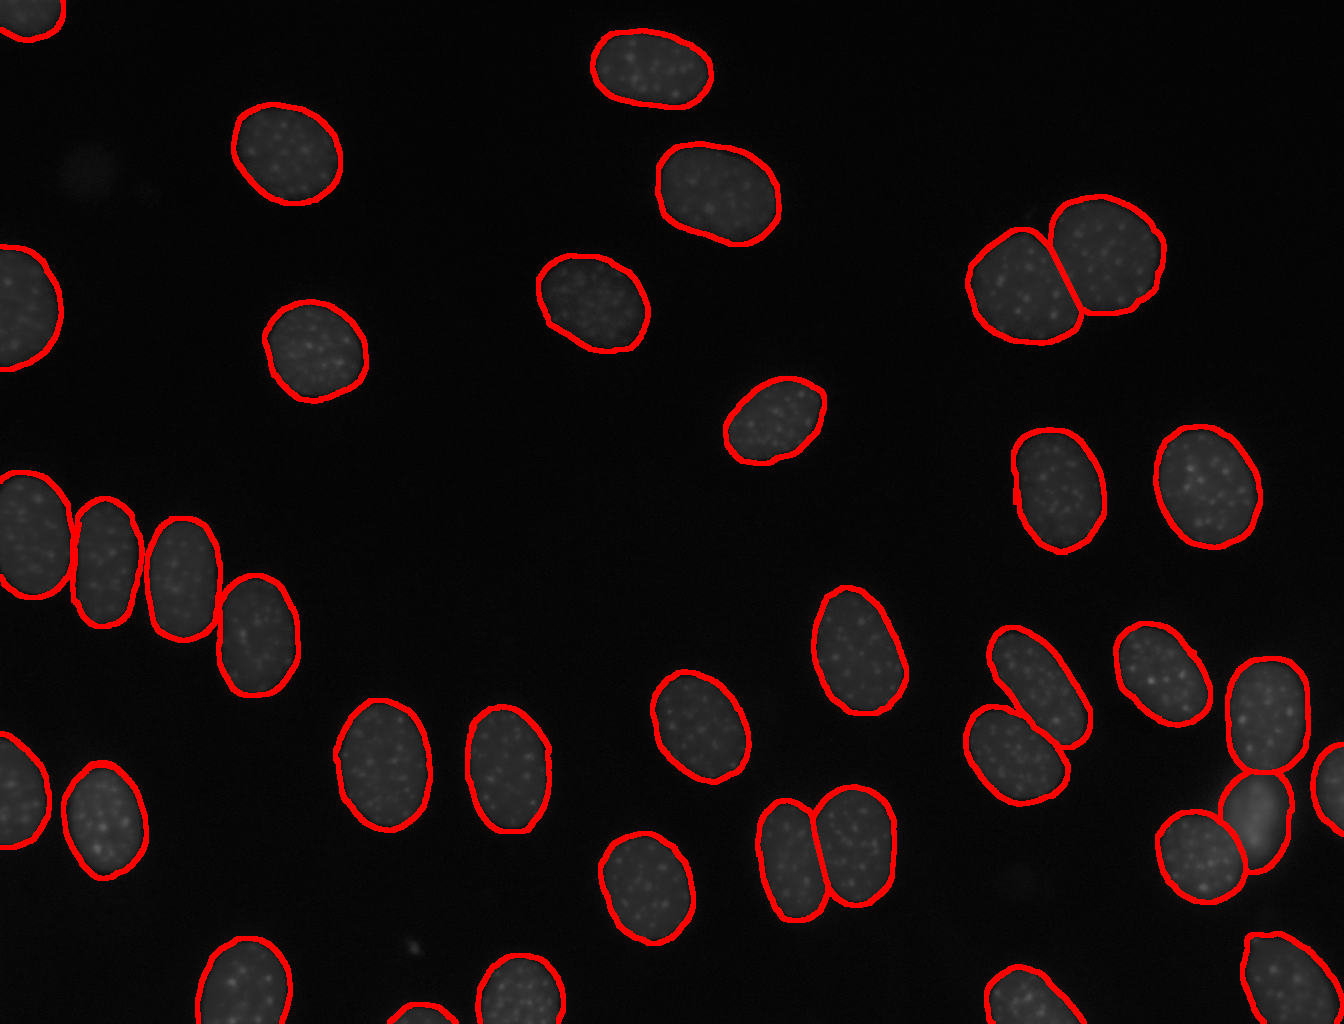
\includegraphics[width=.8\textwidth]{dna}

\end{frame}

\begin{frame}[fragile]
\frametitle{Negative examples}

Simply mix up the segmentation:\\
use image $i$ and the mask $i+1$.
\end{frame}

\begin{frame}[fragile]

\begin{overprint}%
\centering%
\only<1>{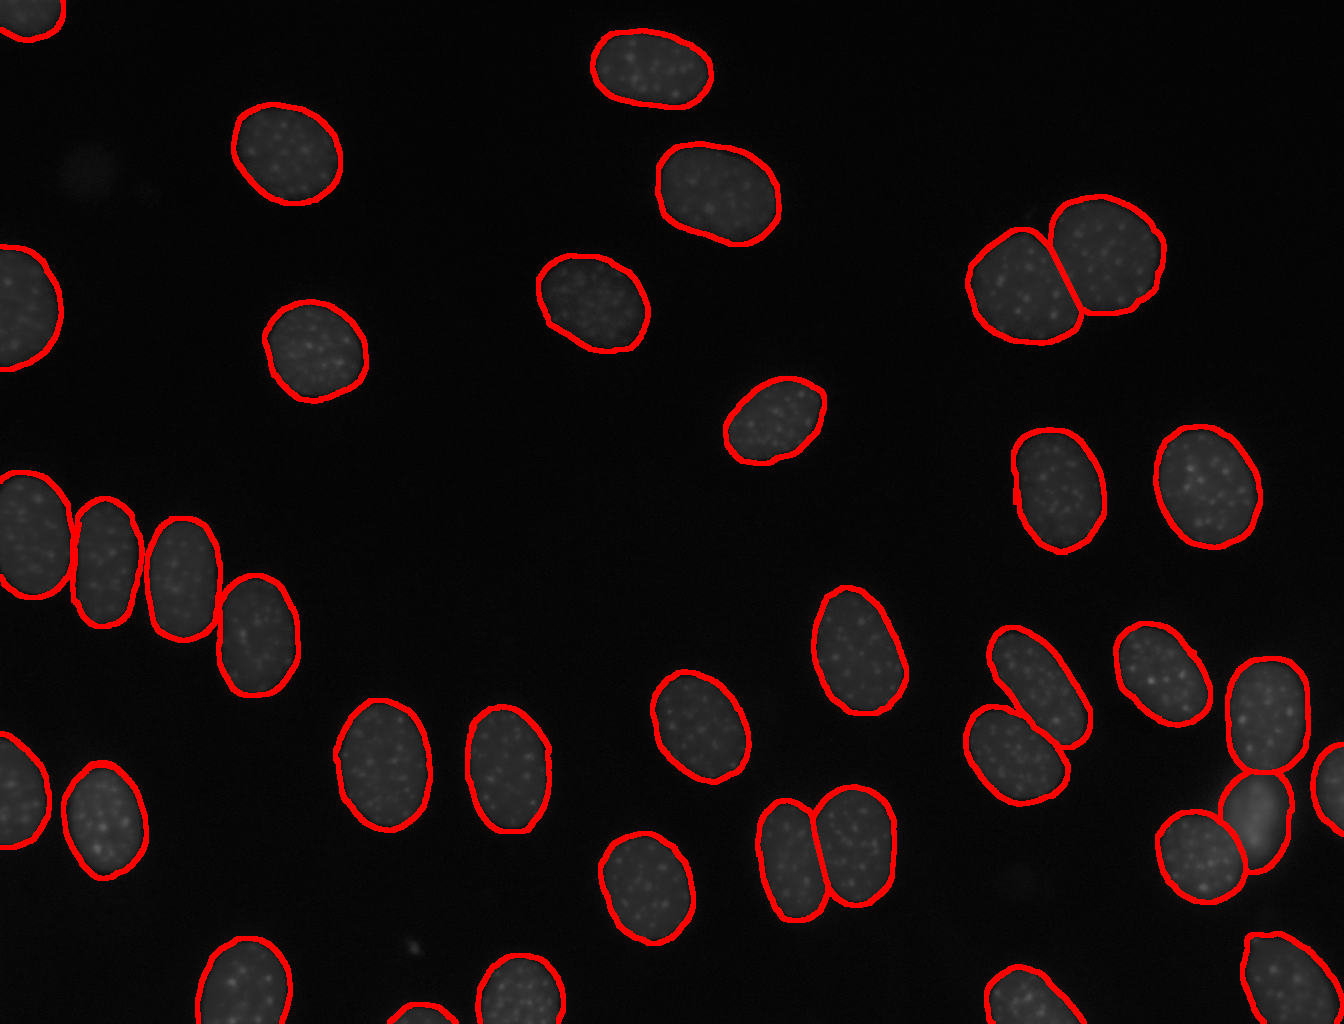
\includegraphics[width=.8\textwidth]{dna}}%
\only<2>{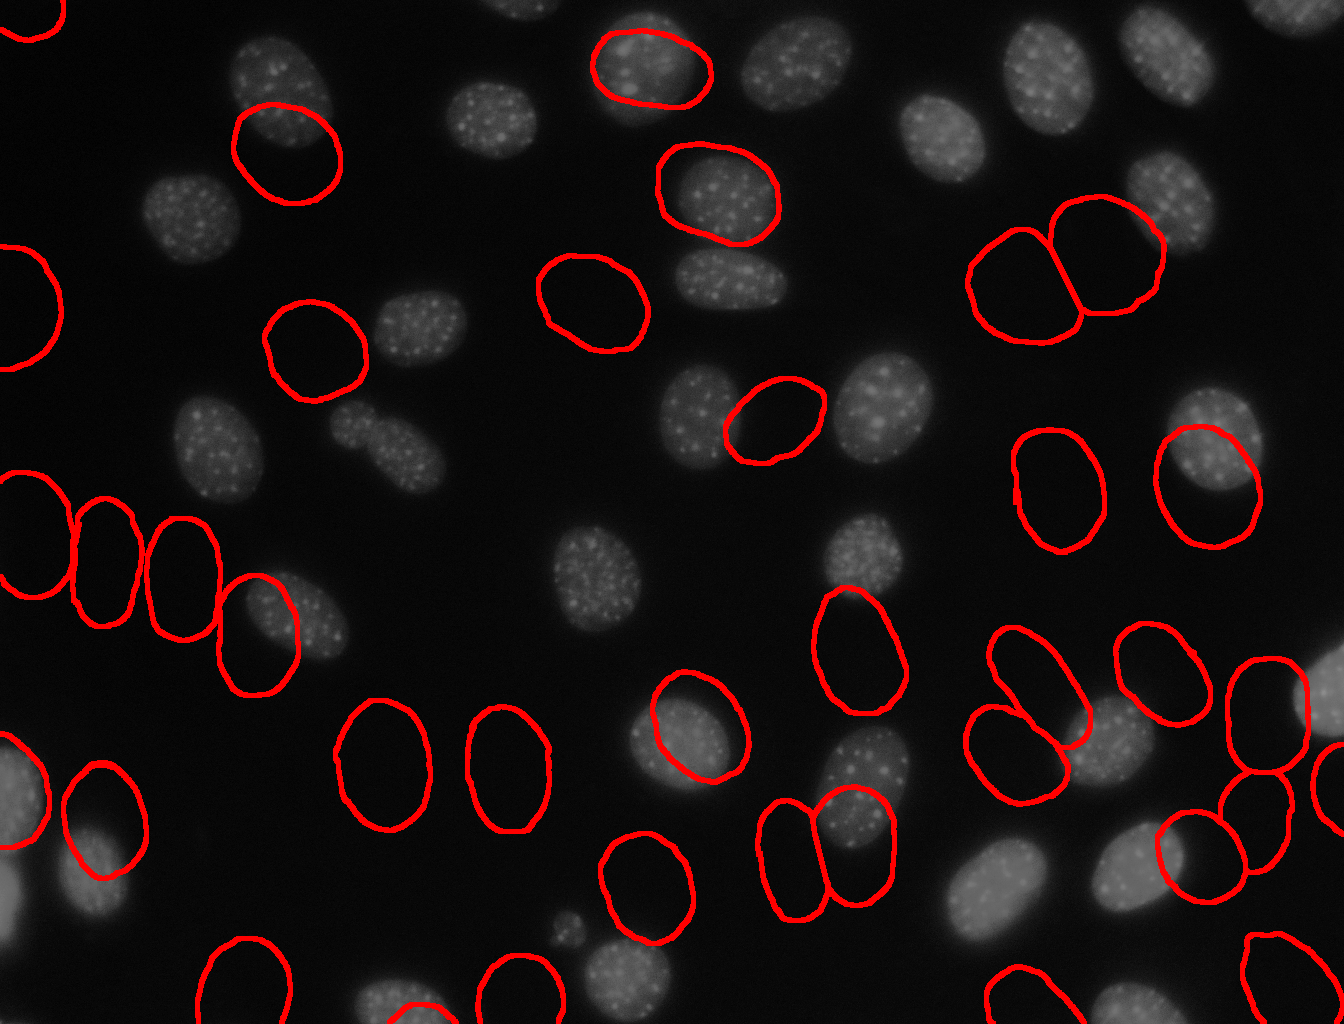
\includegraphics[width=.8\textwidth]{dna2}}%
\par%
\end{overprint}

\end{frame}



\begin{frame}[fragile]
\frametitle{Conclusions}

\begin{itemize}
\item Choose sensible options, but leave optimising to the machine.
\item Replace tunable parameters by learned weights.
\end{itemize}

\end{frame}

\end{document}

